\documentclass{article}
    % General document formatting
    \usepackage[margin=0.7in]{geometry}
    \usepackage[parfill]{parskip}
    \usepackage[utf8]{inputenc}
    
    % Related to math
    \usepackage{amsmath,amssymb,amsfonts,amsthm}
\usepackage{graphicx}
%\usepackage{subfig}
%\usepackage{subfigure}
\usepackage{caption}
\usepackage{subcaption}
\usepackage{listings}

\usepackage{titling}
%\usepackage{lipsum}

\usepackage{titlesec}

\titleformat*{\section}{\large\bfseries}
\titleformat*{\subsection}{\large\bfseries}
%\titleformat*{\subsubsection}{\large\bfseries}
%\titleformat*{\paragraph}{\large\bfseries}
%\titleformat*{\subparagraph}{\large\bfseries}
\titlespacing\section{0pt}{6pt plus 3pt minus 2pt}{0pt plus 2pt minus 2pt}
\titlespacing\subsection{0pt}{6pt plus 3pt minus 2pt}{0pt plus 2pt minus 2pt}
\titlespacing\subsubsection{0pt}{6pt plus 3pt minus 2pt}{0pt plus 2pt minus 2pt}

\pretitle{\begin{center}\large\bfseries}
\posttitle{\par\end{center}\vskip 0.01em}
\preauthor{\begin{center}\Large\ttfamily}
\postauthor{\end{center}}
\predate{\par\normalsize\centering}
\postdate{\par}

%\title{GI Assignment 3: A study of \textit{RB1} variation and regulation}
%\date{\today}

\begin{document}

%\maketitle

\begin{center}
\textbf{\Large{\centering{GSA Assignment: Markov Chains and Hidden Markov Models}}}\\
\vspace{0.8mm}
\textbf{\textit{\small{USN: 303039534}}}
\end{center}
\vspace{1.3mm}

\textbf{\large{1.}}

A function \textit{writemats()} has been written which takes a parameter K and writes a random KxK transition matrix and 1xK initial distribution subject to normalization.
A further function \textit{MC()} takes the filenames of two such matrices together with a chain length N, and generates N elements of a Markov Chain with the specified transition matrix and initial distribution.
Code for both of these functions as well as all other functions written for this assignment can be can be found in the appendix.

As an example, we generate a random transition matrix and initial distribution with K = 3 and obtain the following parameters:

\[
A = 
\begin{bmatrix}
   0.544 &  0.239 &  0.216 \\
   0.323 &  0.216 &  0.461 \\
   0.082 & 0.431 & 0.487 \\
\end{bmatrix}
\]

\[
\mu^0 = 
\begin{bmatrix}
   0.792 \\
   0.100  \\
   0.108  \\
\end{bmatrix}
\]

Using these parameters, we generate a Markov Chain of length 1000 and plot the first 100 elements in figure \ref{fig:MC}.


\begin{figure}[h]
\centering
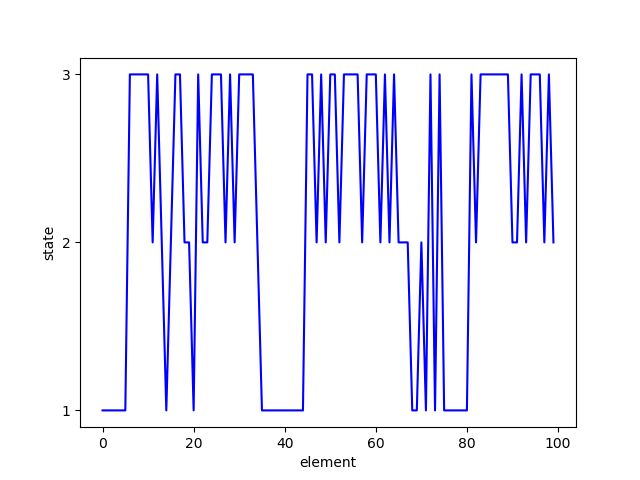
\includegraphics[width = 0.5\linewidth, trim={0 0 0 0}, clip=true]{MC.png}
\caption{First 100 elements of random Markov chain}
\label{fig:MC}
\end{figure}

We find that the model spends 32.1\%, 29.1\% and 38.8\% of the time in states 1, 2 and 3 respectively.
We can also calculate the hypothetical equilibrium distribution, $\bf{\pi}$, of the chain as the distribution for which
\begin{equation}
\pi^{T} \text{A} = \pi^T
\end{equation}
We find this as the eigenvector of $\text{A}^T$ corresponding to an eigenvalue of 1. This equilibrium distribution is
\[
\pi = 
\begin{bmatrix}
   0.291 \\
   0.309  \\
   0.400  \\
\end{bmatrix}
\]

We thus see that our simulated distribution of states is somewhat similar to the equilibrium distribution, but with a bias towards state 1 from starting in state 1 with a high $\text{A}_{11}$ value.


\textbf{\large{2.}}

For a Markov Chain with transition matrix $A$ and initial distribution $\mu_0$, the probability of observing a given sequence of state indices $x_0^N$ is
\begin{equation}
P(x_0^N) = \mu_0(x_0) * \prod_{i, j}{A_{ij}^{n_{ij}}}
\end{equation}
Where $n_{ij}$ is the number of transitions from state i to state j.

We can calculate the maximum likelihood Markov chain transition matrix and initial distribution by maximizing the log of this probability subject to the constraint that each row of the transition matrix must add to 1 since the probability of going from any state i to some state is 1. We do this using Lagrange multipliers:

\begin{equation}
\mathcal{L} =\mu_0(x_0) + \sum_{i, j}{n_{ij}*\log{A_{ij}}}  - \sum_i{\lambda_i * (\sum_j{A_{ij}}-1)}
\end{equation}
\begin{equation}
\dfrac{\partial \mathcal{L}}{\partial A_{ij}} =  0
\end{equation}

This gives

\begin{equation}
\dfrac{n_{ij}}{A_{ij}} = \lambda_i = \sum_j{n_{ij}} 
\end{equation}

From the constraint equations.
We thus estimate the most likely transition matrix elements given our sequence as 

\begin{equation}
A_{ij} = \dfrac{n_{ij} }{ \sum_j{n_{ij}} }
\end{equation}
where $n_{ij}$ is the number of transitions from state i to state j. the Maximum likelihood transition probability  from state i to state j is thus the proportion of total transitions from state i that go to state j.

We also have 
\begin{equation}
\dfrac{\partial \mathcal{L}}{\partial \mu_0(i)} = 0
\end{equation}

This gives $\mu_0(i) = \delta(i, x_0)$. Given a single Markov chain where we only have a single data point from which to infer an initial distribution, the initial distribution is thus 1 for whichever state occurs first and zero for all other states.

A function \textit{MLE()} has been written that performs a maximum likelihood estimation given a state space and a set of Markov chain state indices. 
As an example, we perform a maximum likelihood estimation on the chain generated in part 1 above and arrive at the following transition matrix and initial distribution:


\[
A_{MLE} = 
\begin{bmatrix}
   0.609 &  0.191 &  0.200 \\
   0.341 &  0.244 &  0.415 \\
   0.086 & 0.447 & 0.477 \\
\end{bmatrix}
\]

\[
\mu^0_{MLE} = 
\begin{bmatrix}
   1.000 \\
   0.000  \\
   0.000  \\
\end{bmatrix}
\]

As expected, the initial distribution is 1 for state 1 and zero for states 2 and 3 since our chain starts in state 1 (figure \ref{fig:MC}). A better estimate could be obtained by generating multiple chains and averaging the initial distribution ocer these.
The estimated transition matrix looks similar to the real transition matrix from part 1., albeit with $\text{A}_{11}$ being somewhat higher than expected. Such errors are due to the inherently stochastic nature of the chain and could be mitigated by performing maximum likelihood estimation on a longer chain or averaging over multiple chains.

\textbf{\large{3.}}

We proceed to implement a function \textit{HMC()} which generates a Markov chain of length N using \textit{MC()} and uses this as a hidden chain to generate an observed chain given an emission matrix \textbf{B}.
We then use \textit{HMC()} to generate a chain of 115 hidden and emitted states using the parameters given in the assignment ($\theta_{ass}$) and plot these in figure \ref{fig:ho}.


\begin{figure}[h]
\centering
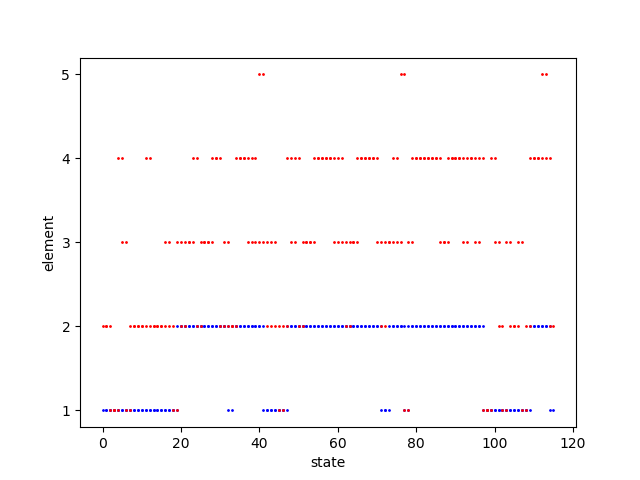
\includegraphics[width = 0.5\linewidth, trim={0 0 0 0}, clip=true]{ho.png}
\caption{115 hidden (blue) and emitted (red) states for a Markov chain generated with the parameters given in the assignment ($\theta_{ass}$).}
\label{fig:ho}
\end{figure}

$\theta_{ass}$ is defined by

\begin{equation}
S_{ass} = {0,1},V_{ass} = {1,2,3,4,5}
\end{equation}
\begin{equation}
\text{A}_{ass} = \begin{bmatrix} 0.8\,\, 0.2 \\ 0.1\,\, 0.9 \end{bmatrix}
\text{B}_{ass} = \begin{bmatrix} 0.2\,\, 0.5\,\, 0.2\,\, 0.1\,\, 0.0 \\ 0.0\,\, 0.1\,\, 0.4\,\, 0.4\,\, 0.1 \end{bmatrix}
\mu_{0, ass} = [0.5\,\, 0.5]
\end{equation}

We see in figure \ref{fig:ho} that there is a bias towards hidden state 2 over hidden state 1 as we expect from inspection of $\text{A}_{ass}$. We also see that hidden state 1 leads to a higher proportion of emitted states 1 and 2 whereas hidden state 2 leads to a higher proportion of emitted states 3, 4 and 5 as expected from inspection of $\text{B}_{ass}$.

\textbf{\large{4.}}

Writing the emitted sequence from part 3. to a file emitted.txt, we further implement the scaled forward algorithm in the function \textit{forward()} to calculate the probability of observing this sequence $y_0^N$ given $\theta_{ass}$.

We first define the parameters $\{\alpha_n(i)\}$ as

\begin{equation}
\alpha_n(i) = P(y_0^n, x_n=i) = \sum_j{\alpha_{n-1}(j) * B_i(V_n) * A_{ji}}
\end{equation}
This recursion is initialized by
\begin{equation}
\alpha_0(i) = \mu_0(i) * B_i(V_0)
\end{equation}
After calculating $\alpha$ at every step of the chain, we can proceed to calculate the probability of observing a sequence of emitted states as
\begin{equation}
P(y_0^N) = \sum_i(P(y_0^N, x_N=i)) = \sum_i{\alpha_N(i)}
\end{equation}

Since $\alpha_n$ becomes progressively smaller with n, underflow can become a problem and we therefore implement a scaled version of the forward algorithm where we normalize each set of $\alpha$ values using normalization constants $c_n = P(y_n | y_0^{n-1})$ such that

\begin{equation}
\hat{\alpha}_n(i) = \dfrac{ \alpha_n(i) }{ \prod_{k=0}^n{c_k}} = \dfrac{ \alpha_n(i) }{ \sum_j{\alpha_n(j)} }
\end{equation}
This prevents underflow and allows us to calculate the total log likelihood of observing $y_0^N$ as
\begin{equation}
\log{P} = \log{\prod_n{c_n}} = \sum_n{\log{c_n}}
\end{equation}

For the chain in figure \ref{fig:ho} we obtain log10p = -69.545 and thus p = 2.851e-70. In the present case, the chain is sufficiently small that underflow is not an issue in Julia, and we thus validate our implementation using the un-scaled algorithm which gives the same probability.

We also implement the backward algorithm for future use in the Baum-Welch algorithm.
Here we define
\begin{equation}
\beta_n(i) = P(y_{n+1}^N, x_n=i) = \sum_j{\beta_{n+1}(j) * B_j(V_{n+1}) * A_{ij}}
\end{equation}
This recursion is initialized by
\begin{equation}
\beta_N(i) =1
\end{equation}

To prevent underflow, we use the same scaling factors as in the forward algorithm such that
\begin{equation}
\hat{\beta}_n(i) = \dfrac{ \beta_n(i) }{ \prod_{k=n+1}^N{c_k} }
\end{equation}

We also use the $\beta$ values from the backward algorithm to check that for all n
\begin{equation}
\sum_i{\alpha_n(i) * \beta_n(i)} = \sum_i{ P(Y_0^n, x_n = i | \Theta) * P(Y_(n+1)^N | x_n = i, \Theta) } = \sum_i{ P(Y_0^N, x_n = i | \Theta)  } = 1 
\end{equation}
 This further validates the present implementation of the forward-backward algorithm.


\textbf{\large{5.}}

We download the \textit{S. cerevisiae} chromosome III from Ensembl and quantify the GC content in 100bp windows using the functions \textit{get\_brackets()} and \textit{calc\_GC()}.

To convert the calculated GC content to emission states from the model in part 3, we need to generate a binning scheme with five bins. We therefore generate a Hidden Markov Chain from $\theta_{ass}$ with 100,000 elements and calculate the frequency of each state [1:5]. The cumulative frequencies are 0.065, 0.297, 0.631, 0.932 and 1.0.
We then plot a cumulative distribution of the GC content in the yeast chromosome (figure \ref{fig:cum}).

\begin{figure}[h]
\centering
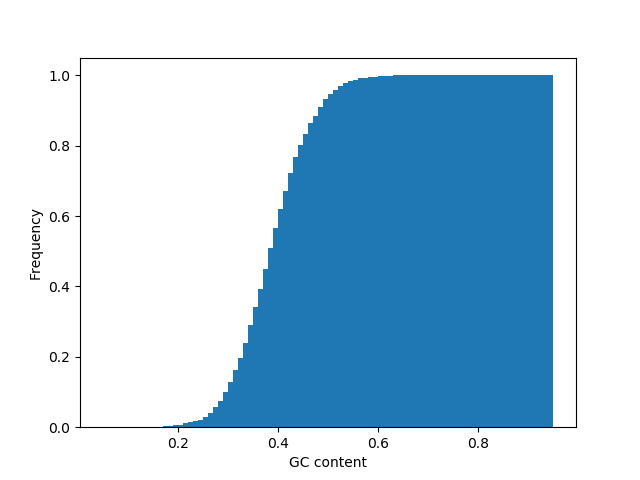
\includegraphics[width = 0.5\linewidth, trim={0 0 0 0}, clip=true]{cumulative_GC.png}
\caption{Cumulative distribution of GC content}
\label{fig:cum}
\end{figure}

By matching these two cumulative distributions, we arrive at the following upper bounds of GC content in a window to correspond to each state 1-5: [0.275, 0.345, 0.405, 0.495, 1.0].

We feed these parameters to the function \textit{GC\_to\_state()} together with the sequence of 3167 calculated GC contents for the 3167 windows and return a sequence of 3167 observed states $s_n \in [1:5]$.

We use this sequence of emitted states as an input to \textit{forward()} together with $\theta_{ass}$ to calculate the probability of observing this particular sequence. In this case underflow does become a problem, and we therefore use the scaled algorithm to calculate the probability which gives a log likelihood of
log10(P) = -1864.385.

\textbf{\large{6.}}

In the Baum-Welch algorithm, we start with a set of initial parameters and define

\begin{equation}
\gamma_n(i) = P(x_n=i | y_0^N) = \dfrac{P(x_n=i, y_0^N)}{P(y_0^N)} = \dfrac{\alpha_n(i) * \beta_n(i)}{\sum_j{\alpha_n(j) * \beta_n(j)}}
\end{equation}

\begin{equation}
\xi_n(i,j) = P(x_n=i , x_{n+1} = j| y_0^N) = \dfrac{\alpha_n(i) * A_{ij} * \beta_{n+1}(j) * B_j(V_{n+1})}{\sum_i{\sum_j{\alpha_n(i) * A_{ij} * \beta_{n+1}(j) * B_j(V_{n+1})}}}
\end{equation}

After calculating $\{\alpha_n\}$ and $\{\beta_n\}$ for each step in the chain of emitted states using the forward algorithm with $\theta_{init}$, we also calculate all $\{\gamma_n\}$ and $\{\xi_n\}$. Using these quantities, we can calculate expected transition frequencies and thus expected parameters $\tilde{\text{A}}$, $\tilde{\text{B}}$ and $\tilde{\mu_0}$:

\begin{equation}
\tilde{\mu}_0(i) = \gamma_1(i)
\end{equation}
\begin{equation}
\tilde{\text{A}}_{ij} = \dfrac{\sum_{n=0}^{N-1}{\xi_n(i,j)}}{\sum_{n=0}^{N-1}{\gamma_n(i)}}
\end{equation}
\begin{equation}
\tilde{\text{B}}_i(V_k) = \dfrac{\sum_{n=0}^{N}{\delta(v_k, v_n) * \gamma_n(i)}}{\sum_{n=0}^{N}{\gamma_n(i)}}
\end{equation}

Where $\delta$ is the delta function.

$\tilde{\mu}_0$, $\tilde{\text{A}}$ and $\tilde{\text{B}}$ will generally be different from the initial parameters A, B and $\mu_0$ used to estimate $\{\alpha_n\}$, $\{\beta_n\}$, $\{\gamma_n\}$ and $\{\xi_n\}$. We can therefore calculate new values for these quantities, which in turn give us a new set of model parameters etc. By iteratively updating the model parameters until they remain stationary, we find a local maximum in parameter space and thus a set of new optimum parameters for the given model and emitted sequence.


We implement the Baum-Welch algorithm in the function \textit{baum\_welch()} with a default convergence threshold of 0.0001 for the 2-norm of a vector of the change in all model parameters. That is, we measure convergence by the parameters becoming stationary rather than the log likelihood becoming stationary, but these are of course related.

To update the parameters for the model in part 3, we use $\theta_{ass}$ as initial parameters. 
After running the Baum-Welch algorithm, we arrive at an optimum log10p = -1821.103 for the emission sequence in part 5.
That is, after running the Baum-Welch algorithm, we obtain a set of parameters that makes this particular emitted sequence 43 orders of magnitude more likely than it was with our initial parameters.
The optimum parameters are:
\[
A = 
\begin{bmatrix}
 0.939 &  0.061\\
 0.120 & 0.880\\
\end{bmatrix}
\]
\[
B = 
\begin{bmatrix}
 0.085 & 0.334  & 0.399 & 0.181 & 0.000\\
 0.000  &    0.032 & 0.197 & 0.567 &  0.204\\
\end{bmatrix}
\]
\[
\mu_0 = 
\begin{bmatrix}
 0.0\\
 1.0\\
\end{bmatrix}
\]

However, the Baum-Welch algorithm can be sensitive to initial parameters, and we therefore validate our result by generating 100 random sets of initial parameters for the algorithm with the function \textit{test\_welch()}. This gives an optimum log10p of -1818.783, which is slightly better than what we observed using $\theta_{ass}$ as initial parameters.
The optimum parameters calculated by \textit{test\_welch} are:

\[
A = 
\begin{bmatrix}
 0.954  &  0.046\\
 0.083  & 0.917\\
\end{bmatrix}
\]

\[
B = 
\begin{bmatrix}
 0.082 &  0.335  & 0.400 & 0.182 & 0.001\\
 0.011 & 0.047 &  0.206  & 0.544 & 0.191\\
\end{bmatrix}
\]

\[
\mu_0 = 
\begin{bmatrix}
 0.0\\
 1.0\\
\end{bmatrix}
\]

A likely reason for the discrepancy is that with $\text{B}_{ass}$, we force B1(5) and B2(1) to be zero, thus decreasing the number of degrees of freedom available for optimization. By relaxing this constraint, we arrive at both of these parameters being slightly higher than zero, and this results in a slightly better fit.

When inspecting the list of 100 log10p values converged to, we observe that all of our simulations converge to one of two local maxima at logp = -1818.78 and logp = -1946.23. This illustrates the potentially large effect of the choice of initial conditions and thus the importance of verifying results with different initial conditions.
Even after running 100 simulations, we do not know for sure if we have in fact found the global maximum or merely local maxima that are commonly converged to in a Baum-Welch framework.
One way to investigate this further would be to implement a metadynamics-like algorithm where we prevent reconvergence to maxima already found, but that is beyond the scope of the present assignment

We can also alter the binning procedure from the one in part 5 where we match the state distribution expected from $\theta_{ass}$.
Another straightforward approach would be to bin GC content such that states 1-5 become equally frequent in the yeast chromosome.
Using this binning procedure and running \textit{test\_welch()} leads to a best fit with optimum log10p = -2070.062 from 100 simulations, which is significantly different from what we observed with the previous binning scheme.
This suggests that the choice of binning can strongly affect the result, calling for a potential optimization of the binning scheme. However, this is a 4-parameter optimization that is beyond the scope of the present assignment (although it could be implemented relatively simply using steepest descent with empirical gradients or quasi-newton optimx	ization with empirical gradient and hessian if the log10p landscape is well-behaved).

We could also achieve better fits by altering the number of free parameters further and allowing for e.g. more than 2 hidden states and more than 5 observed states. This is a rather difficult hyperparameter optimization problem which balances overfitting and predictive power and is beyond the scope of the present assignment. However, it is an interesting and important problem both in the field of Hidden Markov Models and in machine learning more generally.


\textbf{\large{7.}}


To find the most likely sequence of hidden states (the Viterbi path) given an emitted sequence and a set of parameters, we implement the Viterbi algorithm in the function \textit{viterbi()}. In the viterbi algorithm, we define

\begin{equation}
\omega_{n,i} = \log{P(y_0^N, x_0^N)} = \log{P(y_n|x_n = i)} + \max_k{[ \omega_{n-1, k} + \log{P(x_n =i | x_{n-1} = k)}]}
\end{equation}
This recursion is initialized by
\begin{equation}
\omega_{1,i} = \log{\mu_0(i)} + \log{B_i(V_0)} 
\end{equation}

We also store for every element n and state i which previous state lead to $\omega_{ni}$, such that

\begin{equation}
\text{traceback}_{n,i} = \text{argmax}_k [ {\log{P(y_n| i)} + \omega_{n-1,k} + \log{P(i |  k )}  } ] 
\end{equation}

After calculating all $ \{ \omega_{n,i} \} $, we can find the Viterbi path using traceback

\begin{equation}
\text{path}[N] = \text{argmax}_i(\omega_{N,i})
\end{equation}
\begin{equation}
\text{path}[n] = \text{traceback}[n+1, \text{path}[n+1]]
\end{equation}

We proceed to find the Viterbi path using the optimized parameters from the Baum-Welch optimization with initial parameters $\theta_{ass}$.
This results in a Viterbi path with a log likelihood of -1896.813 for the most likely sequence of hidden states.

We plot the Viterbi path together with the actual GC content for 100 windows along the yest chromosome in figure \ref{fig:viterbi}. In this figure, the GC content has been scaled to a range of [0:3] for plotting together with the hidden Markov states. This corresponds to a real range of GC contents of [0.11:0.63].
As also observed in figure \ref{fig:ho} we see that state 1 generally corresponds to lower GC contents and state 2 to higher GC contents.
We also see that there are generally longer stretches of state 1 and state 2 rather than rapid oscillations between the two. This is a result of the transition matrix having large diagonal elements.

\begin{figure}[h]
\centering
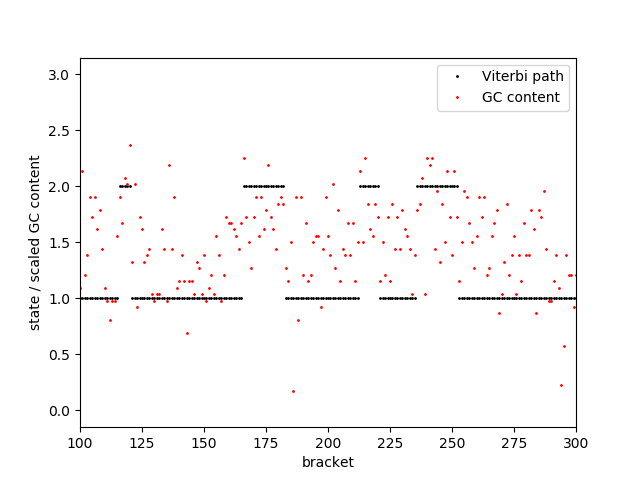
\includegraphics[width = 0.5\linewidth, trim={0 0 0 0}, clip=true]{viterbi_path.png}
\caption{Viterbi path (black) and GC content scaled to a range of 0 to 3 for position 10,000 to 30,000 of \textit{S. cerevisiae} chromosome III}
\label{fig:viterbi}
\end{figure}


Utility: e.g. euchromatin vs. heterochromatin. Transcriptionally active vs passive. ORF finding.

gene finding; higher GC content due to evolutionary constraints?



\section*{Appendix (code)}

\lstset{basicstyle=\footnotesize}

\large{File: gsa.jl}
\lstinputlisting[language=python]{gsa.jl}

\large{File: markov\_chains.jl}
\lstinputlisting[language=python]{markov_chains.jl}

\large{File: anal\_GC.jl}
\lstinputlisting[language=python]{anal_GC.jl}

\large{File: forward.jl}
\lstinputlisting[language=python]{forward.jl}

\large{File: viterbi.jl}
\lstinputlisting[language=python]{viterbi.jl}

\end{document}

